\documentclass{article}
\usepackage{tikz}
\usetikzlibrary{positioning,fit,arrows.meta,decorations.pathreplacing}

\begin{document}

\begin{figure}[h]
    \centering
    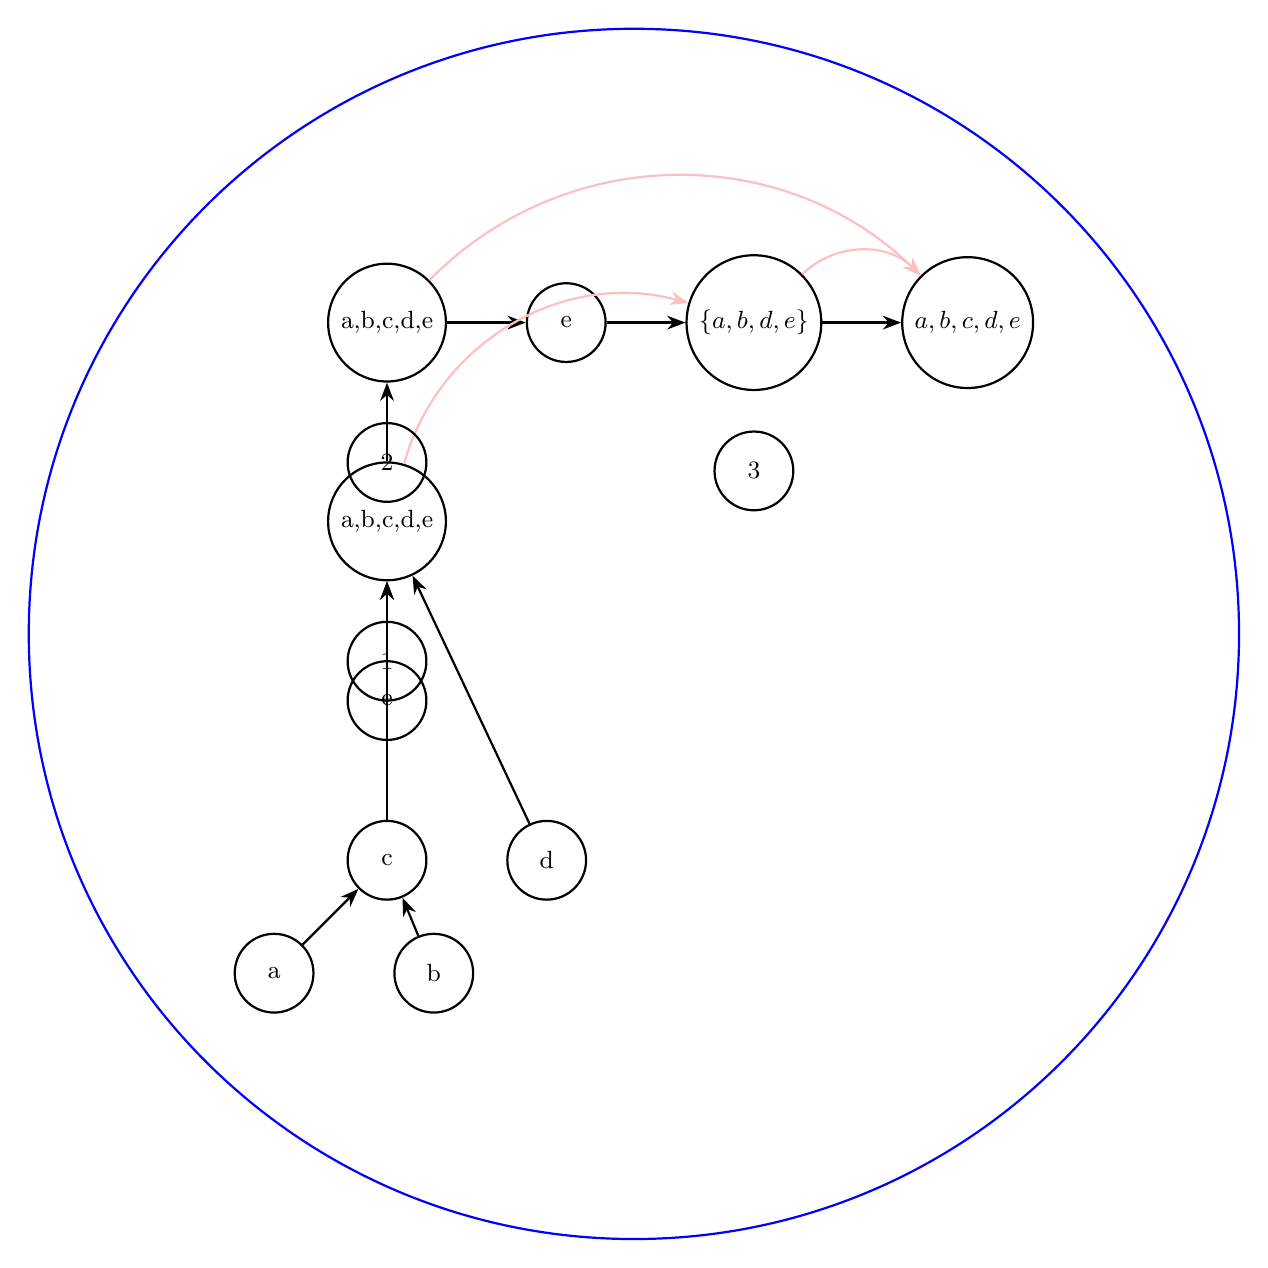
\begin{tikzpicture}[
        node distance = 1cm,
        every node/.style = {draw, circle, minimum size=1cm},
        >=Stealth,
        thick,
        font=\small
    ]
    
    % Define nodes
    \node (a) {a};
    \node[right=of a] (b) {b};
    \node[above right=of a] (c) {c};
    \node[right=of c] (d) {d};
    \node[above=of c] (e) {e};
    \node[above=of e] (root) {a,b,c,d,e};
    \node[above=of root] (root2) {a,b,c,d,e};
    \node[right=of root2] (e2) {e};
    \node[right=of e2] (root3) {$\{a,b,d,e\}$};
    \node[right=of root3] (root4) {$a,b,c,d,e$};
    
    % Draw edges
    \draw[->] (a) -- (c);
    \draw[->] (b) -- (c);
    \draw[->] (c) -- (root);
    \draw[->] (d) -- (root);
    \draw[->] (e) -- (root);
    \draw[->] (root) -- (root2);
    \draw[->] (root2) -- (e2);
    \draw[->] (e2) -- (root3);
    \draw[->] (root3) -- (root4);
    
    % Draw dashed lines
    \draw[dashed] (root) -- (root2);
    \draw[dashed] (root2) -- (e2);
    \draw[dashed] (e2) -- (root3);
    \draw[dashed] (root3) -- (root4);
    
    % Draw pink arrows
    \draw[->, color=pink] (root) to[bend left=45] (root3);
    \draw[->, color=pink] (root2) to[bend left=45] (root4);
    \draw[->, color=pink] (root3) to[bend left=45] (root4);
    
    % Draw labels for arrows
    \node[below=0.5cm of root] (label1) {1};
    \node[below=0.5cm of root2] (label2) {2};
    \node[below=0.5cm of root3] (label3) {3};
    
    % Draw blue box
    \node[draw=blue, thick, rounded corners, fit=(a) (d) (root) (root2) (e2) (root3) (root4), inner sep=0.5cm] {};
    
    \end{tikzpicture}
    \caption{Visualization of the $\sqrt{n}$-decomposition of the blue group from Figure~\ref{fig:group-partition}. The processes $a,b,c,d,e$ in the group are logically decomposed into a binary tree. The pink arrows visualize the three-round process of relaying operative counts of the two children of the root to the root itself. First, the counts are relayed to all processes in the group (arrow \#1), then the processes send a confirmation if they received the counts (arrow \#2), finally, all in the group transmit the received counts to the higher layer -- the root in this case (arrow \#3). Some processes can be faulty (process $c$ does not communicate, only $\{a,b,d,e\}$) and their values are not guaranteed to be accumulated accurately.}
    \label{fig:decomposition}
\end{figure}

\end{document}